\section{Organizzazione Aziendale}

\subsection{Intro}
Questa parte del programma illustra come un'azienda viene organizzata, come si relazionano funzioni diverse ed aprire una panoramica sulle modalità organizzative di un'azienda.

I contenuti che verrano presentati sono:
\begin{itemize}
	\item Struttura ed elementi costitutivi di un’azienda
	\item Descrizione delle funzioni principali
	\item Tipi di interazioni tra funzioni
	\item \textit{Lean thinking} come approccio organizzativo
\end{itemize}

\subsection{Definizione di Azienda}
Dall'articolo \textbf{2555} del \textit{Codice Civile}, \textit{l’azienda} è il complesso di beni organizzati da un soggetto (imprenditore) per l’esercizio di un’attività economica (impresa).

Mentre dall'articolo \textbf{2082} del \textit{Codice Civile}, \textit{l'imprenditore} è chi esercita professionalmente un’attività economica organizzata al fine della produzione o dello scambio di beni o servizi.

L'obiettivo principale di un'azienda è, attraverso un insieme di risorse, quello di svolgere processi di acquisizione e produzione di beni e/o servizi da scambiare con entità esterne al fine di conseguire un \textbf{reddito}.
\subsection{Progettazione}
La progettazione nello sviluppo di prodotti ricerca la migliore risposta, in termini di prodotto, alle aspettative del cliente. I principali compiti sono:
\begin{itemize}
	\item Definisce la forma del prodotto
	\item Identifica le prestazioni
	\item Disegna i componenti
	\item Ricerca la migliore soluzione “producibile”
	\item Valuta la “funzione” dei componenti
	\item Garantisce la migliore prestazione (globale), entro i limiti di costo assegnati
\end{itemize}

La sviluppo di nuovi prodotti si suddivide in vari step. Fondamentale è partire da un'idea, per poi:
\begin{enumerate}
	\item \textbf{Analisi e Pianificazione preliminare}: Analisi preliminare tecnica, economica, di mercato. Primo piano di prodotto.
	\item \textbf{Concetto e pre-desing}: Bisogni dei clienti, analisi aspetti tecnici ed economici, architettura preliminare.
	\item \textbf{Sviluppo tecnico}: Progettazione di dettaglio, progettazione processi produttivi, primi prototipi.
	\item \textbf{Testing e prove di collaudo}: Test presso i clienti, pianificazione processo produttivo e lancio.
	\item \textbf{Lancio}: Organizzazione lancio, preparazione documentazione di prodotto, comunicazione.
\end{enumerate}

\subsection{Produzione}
La produzione ricerca le migliori soluzioni industriali, in termini di producibilità, costi e qualità.
I principali compiti sono:
\begin{itemize}
	\item Definisce ed ottimizza il ciclo produttivo
	\item Progetta e realizza il sistema produttivo
	\item Definisce la logistica operativa
	\item Ricerca la migliore soluzione negli “acquisti” 
	\item Programma e controlla la prima produzione
	\item Garantisce il prodotto a magazzino
\end{itemize}
\newpage
\subsection{Marketing}
È la funzione d'impresa che identifica i \textbf{BISOGNI}, i \textbf{COMPORTAMENTI}, le \textbf{ASPETTATIVE} ed i \textbf{DESIDERI} (espressi e inespressi) insoddisfatti, che ne definisce l'ampiezza, che determina quali mercati obiettivo l'impresa può meglio servire, che definisce il valore da offrire attraverso prodotti/servizi e i programmi rivolti ai mercati suddetti, che sollecita tutte le componenti dell'azienda a pensare in termini di servizio al cliente e gestione della relazione.

Il \textit{marketing} è l'interfaccia tra azienda e cliente.

\subsubsection{Marketing Strategico}
Analizza i bisogni dei clienti e definisce il mercato di riferimento dell’impresa (orizzonte di riferimento di medio lungo periodo). A causa dell’eterogeneità dei bisogni della clientela, essa deve essere suddivisa o segmentata in gruppi omogenei al loro interno ed eterogenei fra loro.

Il \textit{marketing} strategico è una programmazione di ampio respiro, che può durare pochi mesi o diversi anni, e che ha come obiettivo principale studiare il mercato al fine di ottimizzare gli strumenti di comunicazione e raggiungere obiettivi di maggior guadagno con minor sforzo e in minor tempo.
Ha l’arduo e stimolante compito di portare un concreto vantaggio competitivo all’azienda grazie ad un’attenta pianificazione delle attività di \textit{marketing} e comunicazione.

Attraverso una visione del mercato e dei suoi mutamenti il più possibile completa, un’analisi attenta delle opportunità e dei rischi, è possibile infatti sviluppare una filosofia aziendale orientata al cliente che sia in grado di creare valore tangibile per l’azienda.

La segmentazione del mercato è il processo mediante il quale si suddivide il mercato in un numero limitato di segmenti, ognuno dei quali sufficientemente omogeneo per motivazioni, comportamenti e scelte, ma nello stesso tempo abbastanza differenziato dagli altri.
La scelta fondamentale che caratterizza la strategia di marketing è relativa alla definizione dei mercati di riferimento:
\begin{itemize}
	\item \textit{Marketing} di massa o indifferenziato 
	\item \textit{Marketing} differenziato
	\item \textit{Marketing} concentrato
\end{itemize}
Per la costruzione di tale spazio, si devono identificare i seguenti punti:
\begin{enumerate}[label=\alph*)]
	\item L’identificazione di un insieme di dimensioni che rappresentino gli attributi salienti per i quali i consumatori scelgono un dato prodotto
	\item Una scala di misurazione del valore assegnato
	\item La rappresentazione grafica di questi valori su più dimensioni
\end{enumerate}
Il posizionamento definisce il modo in cui l’impresa e/o il prodotto sono percepiti dagli acquirenti potenziali, in relazione ai concorrenti. Per definire il posizionamento in maniera operativa le imprese individuano uno spazio multidimensionale dove ciascun prodotto o marca occupa una determinata posizione.
I problemi che il marketing strategico risolve sono:
\begin{itemize}
	\item Il piano \textit{marketing} parte dalla definizione di obiettivi organizzativi che siano misurabili e soprattutto chiari, che permettano di fare le giuste scelte di pianificazione.
	\item In prima battuta quindi il marketing strategico permette di fare il punto della situazione e stabilire obiettivi razionali attraverso la determinazione delle aree di \textit{business}.
	\item Grazie ad un piano \textit{marketing} inoltre è possibile individuare nuove opportunità in diversi segmenti di mercato o nel ciclo di vita del prodotto o bisogni ancora non ben individuati nel nostro \textit{target}.
	\item Il piano \textit{marketing} inoltre aiuta a semplificare le strategie adottabili, razionalizzarle e indicare il giusto percorso attraverso la definizione di azioni precise. In poche parole permette di fare ordine nel caos teorico, anche mutando più volte nel corso del tempo, adattandosi al contesto sempre mutevole e strutturando un piano operativo definito e attuabile nei tempi e nei modi giusti.
\end{itemize}

\begin{figure}[h]
	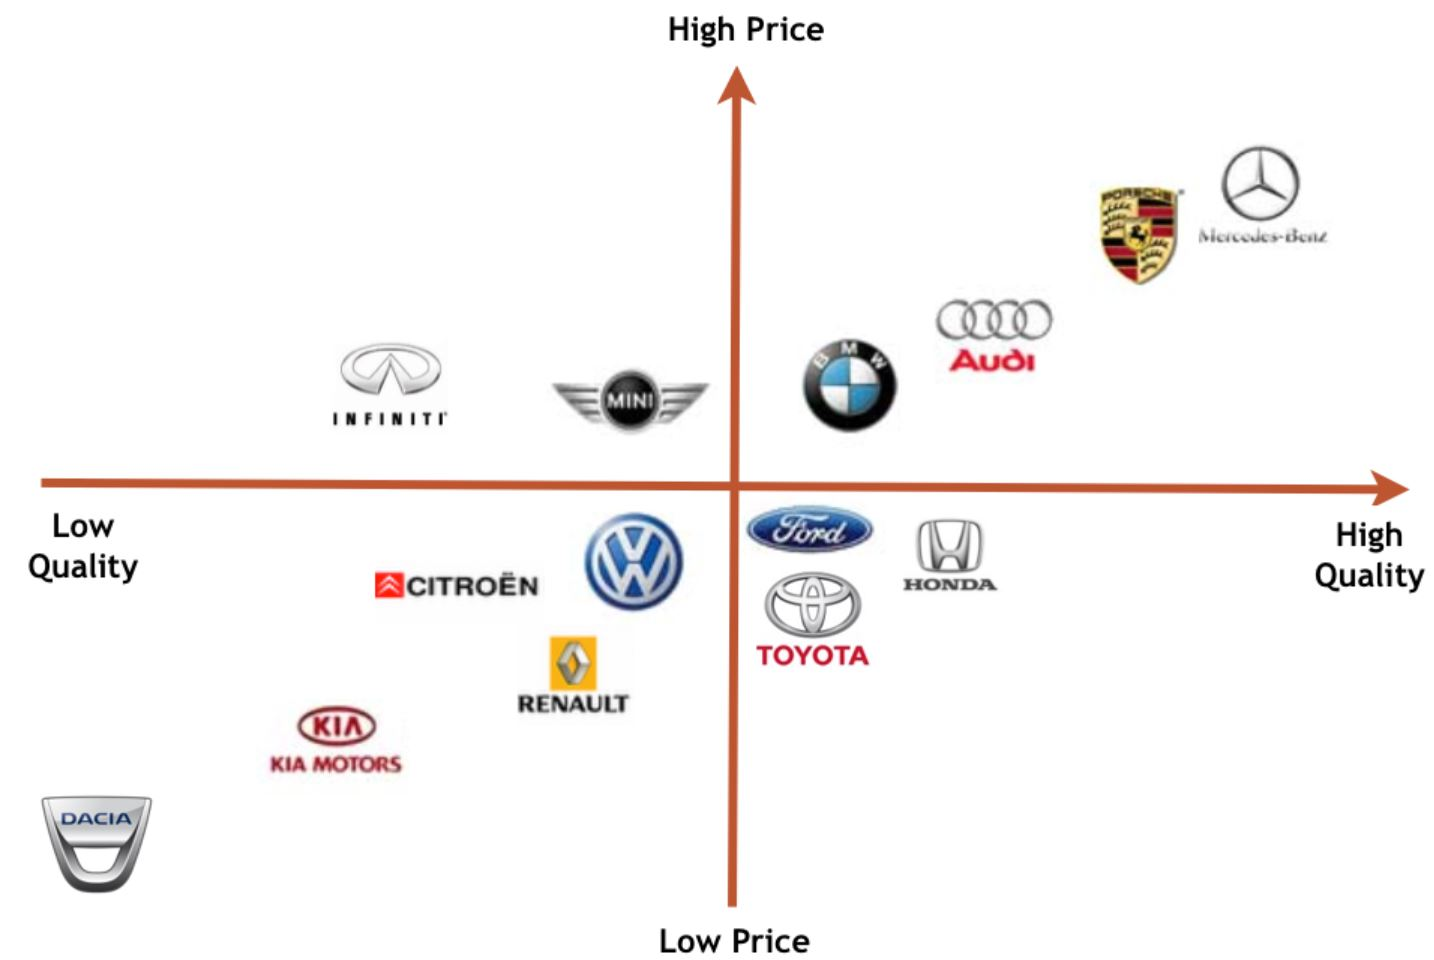
\includegraphics[width=0.6\linewidth]{resources/chapters/OrganizzazioneAziendale/images/mappa-posizionamento.jpg}
	\centering
	\caption{Mappa che raffigura il posizionamento di mercato nel settore automobilistico}
\end{figure}

Il \textit{marketing} strategico si può riassumere in:
\begin{itemize}
	\item Ricerca ed elabora le opportunità di mercato
	\item Definisce i segmenti di mercato
	\item Identifica le aspettative del cliente
\end{itemize}

\newpage
\subsubsection{Marketing Operativo}
Il \textit{marketing} operativo è la parte finale dell’intero processo di \textit{marketing}, a monte del quale ci sono le fasi di marketing analitico e marketing strategico. Solo dopo aver studiato i dati dell’azienda e dei concorrenti e aver pianificato le operazioni da eseguire, arriva il momento dell’azione. La componente operativa (o tattica) del \textit{marketing} ha il compito di realizzare concretamente le strategie definite nelle fasi precedenti, disponendo delle risorse (denaro, professionalità, tecnologia) nel modo più efficace.

\paragraph{Teoria delle 4 P}
\begin{itemize}
	\item \textbf{Prodotto:} le caratteristiche del prodotto o servizio progettato per soddisfare le esigenze di un determinato gruppo (segmento) di consumatori
	\item \textbf{Prezzo:} le politiche di prezzo adottate, il prezzo rappresenta il corrispettivo in denaro che il consumatore è disposto a pagare per fruire di un determinato bene o servizio
	\item \textbf{Placement:} la distribuzione commerciale, ovvero i canali attraverso cui l'impresa porta il prodotto ai diversi \textit{target} di consumatori. Esistono tre tipologie di canali:
		\begin{itemize}
			\item Canale diretto: il consumatore viene raggiunto direttamente dall’azienda senza intermediari. Esso rappresenta la tipica via di distribuzione dei beni strumentali
			\item Canale indiretto breve: il consumatore viene raggiunto con l’intermediazione del dettagliante
			\item Canale indiretto lungo: vi sono più stadi di intermediazione. Il prodotto viene acquistato da un grossista che poi lo rivende ad un dettagliante
		\end{itemize}
	\item \textbf{Promozione:} le attività di comunicazione attraverso cui l'azienda cerca di far conoscere e apprezzare la propria offerta
\end{itemize}

\begin{figure}[h]
	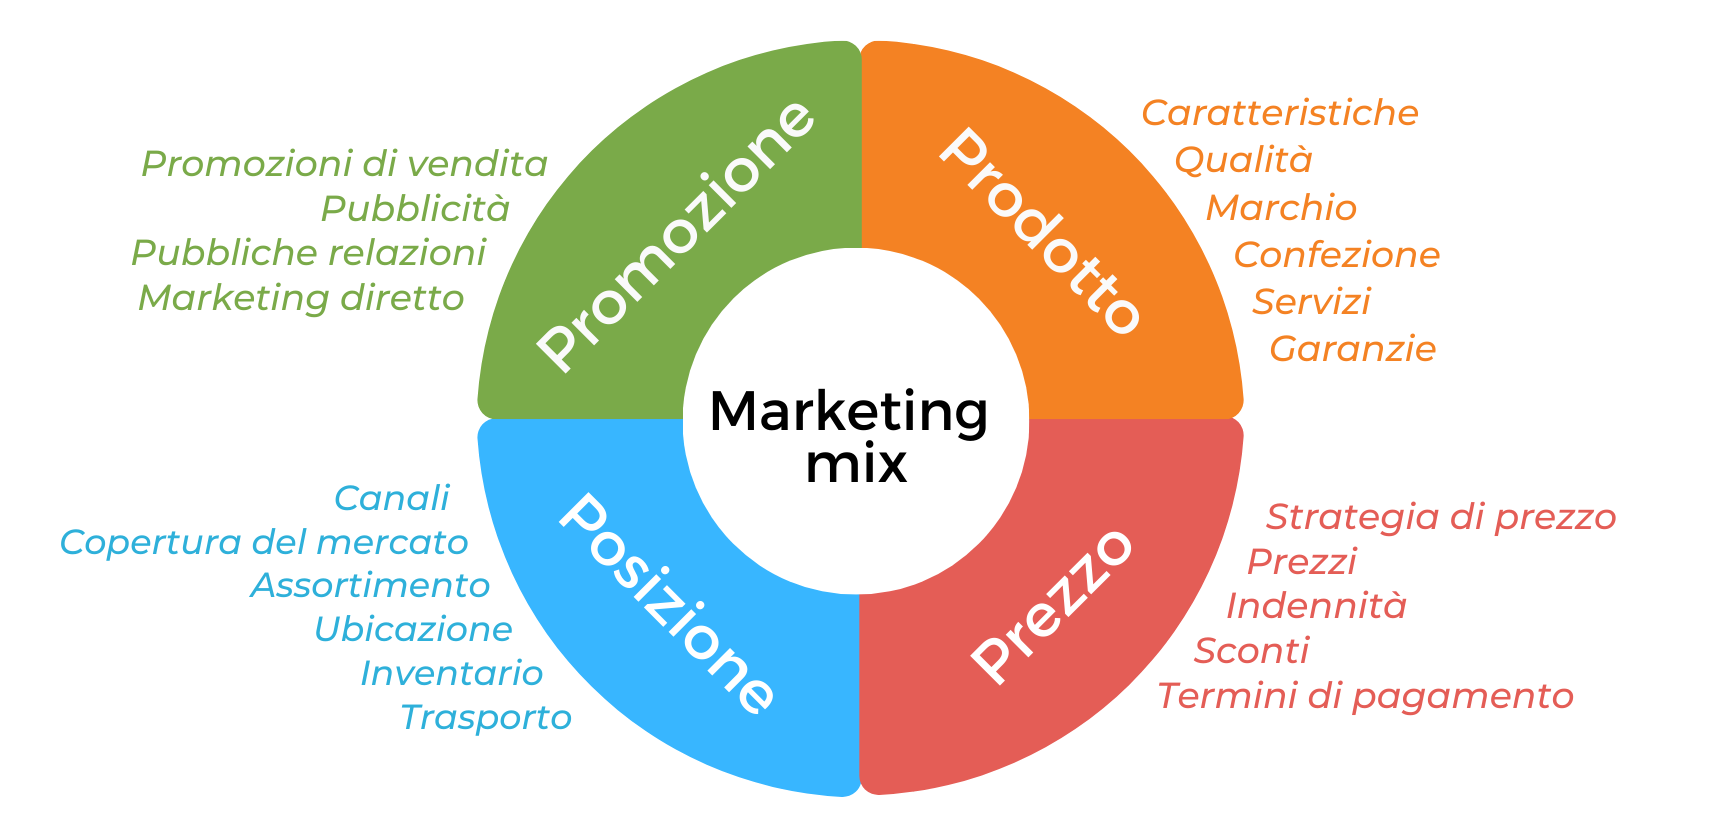
\includegraphics[width=0.7\linewidth]{resources/chapters/OrganizzazioneAziendale/images/pppp.png}
	\centering
	\caption{Riassunto della teoria delle quattro "P"}
\end{figure}
\newpage
\subsection{Filosofia Lean}
Il \textit{lean thinking} nasce come concettualizzazione di un sistema di management collaudato con risultati eccellenti: il \textit{Toyota Production System (TPS)}.

Le sue origini provengono dall’ambito manifatturiero ma oggi è applicato con successo a tutti i processi operativi: progettazione e sviluppo prodotto, logistica e amministrazione.

Tra il 1800 e 1910 il sistema di produzione era organizzato secondo le logiche tipiche dell’artigianato: caratterizzato da bassi volumi di produzione, elevata varietà di prodotti da unicità, scarsa divisione del lavoro e basso coordinamento, assenza di forme di automazione.

Tra il 1910 e il 1950 una nuova forma di capitalismo è emersa in seguito alla concentrazione del capitale industriale e finanziario in grandi imprese, per rispondere alla esigenza di ingenti investimenti in macchinari e impianti.

In queste grandi imprese industriali cominciò a diffondersi la produzione in serie e su larga scala nota come fordismo. Henry Ford\footnote{Dearborn, 30 luglio 1863 – Detroit, 7 aprile 1947 - Imprenditore statunitense, co-fondatore della Ford Motor Company} si ispirò alle teorie di Frederick Taylor\footnote{Germantown, 20 marzo 1856 – Filadelfia, 21 marzo 1915 - Ingegnere ed imprenditore statunitense, famoso per la sua ricerca sul miglioramento dell'efficienza dei metodi produttivi}, l’applicazione dei principi di \textit{“organizzazione scientifica del lavoro”}, di una divisione del lavoro molto spinta basata sull’analisi dei tempi e dei metodi e di un forte ricorso all’automazione, e introdusse per la produzione del modello \textit{Ford T} la catena di montaggio, ottenendo così una produzione di massa, altamente standardizzata, con una notevole diminuzione nei tempi di produzione. La produzione di massa è caratterizzata da una forte integrazione verticale e centralizzazione delle decisioni, un orientamento alla produzione di elevate quantità con alto livello di standardizzazione: l’attenzione non si focalizza sul flusso del materiale o prodotto quanto sulla produzione della maggior quantità possibile. Lo scollegamento dei processi produttivi fa sì che le scorte di semilavorati crescano notevolmente, la produzione non è programmata sulla base della domanda di mercato e i prodotti finiti vengono comunque spinti sulla rete di venditori (\textit{produzione push}).

Il modello sviluppato da \textit{Ford} fu da ispirazione per il sistema di produzione adottato da \textit{Toyota}\footnote{Casa automobilista giapponese} negli anni 40 che lo perfezionò per rispondere alle necessità di flessibilità della produzione e una disponibilità di infrastrutture minore.

Sotto la guida dell’ingegnere capo Taichii Ohono\footnote{Dalian, 29 febbraio 1912 – Toyota, 28 maggio 1990 - Ingegnere giapponese} \textit{Toyota} sviluppò il \textit{TPS} (\textit{Toyota Production System}), un sistema di produzione guidato dai principi di lotta agli sprechi e di miglioramento continuo, caratterizzato da una automazione limitata e flessibile, dalla polifunzionalità degli operatori e da una integrazione a rete.

Il termine \textit{“lean”} è divenuto popolare nel 1990 grazie al libro \textit{“La macchina che ha cambiato il mondo”} di \textit{Womack Jones} e \textit{Roos}. Essi hanno chiaramente illustrato per la prima volta, le notevoli differenze tra il sistema produttivo occidentale e il \textit{TPS}. Hanno definito gli elementi chiave che consentivano delle prestazioni superiori, come \textit{lean production} o produzione snella, snella perché il sistema produttivo giapponese ha permesso di utilizzare meno di tutto – meno sforzo umano, meno investimento di capitali, strutture, meno scorte e tempo – nella produzione, nello sviluppo del prodotto, nella fornitura e nella vendita.

\subsubsection{Concetti base della filosofia Lean}
Alla base del \textit{lean thinking} risiedono dei concetti fondamentali che rivoluzionano la cultura e il modo di operare all’interno dell’azienda:
\begin{itemize}
	\item \textbf{Attenzione al cliente.} La centralità del cliente è il punto di partenza e di arrivo di tutte le attività ed azioni messe in campo dall’azienda nel trasferire, attraverso i propri prodotti e servizi, il valore che il cliente si attende. Il cliente non è solo quello finale, il cliente “interno” è ugualmente importante. Il flusso di informazioni parte dal cliente fino ad arrivare alla ricerca e sviluppo: il dialogo con il cliente è fondamentale per identificare i fabbisogni e definire il valore.
	\item \textbf{Il contributo delle persone.} “Saper fare azienda”, o saper fare bene le cose (concetto giapponese \textit{Monozukuri}), è possibile solo partendo dalla capacità di gestire le persone (\textit{Hitozukuri}): lo sviluppo e il sostegno della competitività aziendale, con l’ottenimento di risultati significativi e duraturi, è possibile solamente con il continuo e costante allineamento del management e di tutte le persone che lavorano nell’azienda verso un obiettivo comune.
	\item \textbf{Lotta agli sprechi.} \textit{MUDA} è il termine giapponese che può essere tradotto come spreco. I \textit{MUDA} consistono in tutte le attività, che impegnano risorse ed energie, che non aggiungono valore al prodotto o al servizio e non danno quindi valore al cliente. Riconoscere gli sprechi è fondamentale per l’applicazione del \textit{lean thinking}.
	\item \textbf{Miglioramento continuo.} \textit{KAIZEN} in giapponese significa miglioramento continuo: nessun processo è perfetto ma può essere sempre migliorato. Tutto il personale dell’azienda, top management, dirigenti, responsabili, fino agli operatori, deve partecipare al processo di miglioramento condividendo obiettivi comuni e definiti.
\end{itemize}

\subsubsection{I 5 passi per la trasformazione Lean}
Nel libro \textit{“Lean Thinking” Womack} e \textit{Jones} hanno individuato i 5 principi chiave che devono essere accolti da una azienda per adottare il \textit{lean thinking}:
\begin{enumerate}
	\item \textbf{Value.} Ripensare al valore dal punto di vista del cliente. Solo una piccola parte delle azioni e del tempo totale che sono impiegate per produrre o fornire un servizio aggiungono effettivo valore per il cliente finale. Risulta quindi fondamentale definire chiaramente il valore di uno specifico prodotto o servizio dalla prospettiva del cliente, così che si possa procedere alla rimozione passo dopo passo di tutte le attività a non valore o \textit{MUDA}. Vengono anche definiti i 7 sprechi da evitare:
		\begin{enumerate}[label=\arabic*.]
			\item \textbf{Processi.} Presenza di operazioni inutili/inefficienti all’interno del ciclo di lavoro (tempi e metodi)
			\item \textbf{Sovrapproduzione.} Realizzare produzione non richiesta o anticipata o non necessaria in quel momento
			\item \textbf{Tempo.} Tempi di attesa dovuti a problemi di bilanciamento e/o mancata sincronizzazione tra le fasi del processo
			\item \textbf{Scorte.} Presenza di scorte eccessive di materiali/attrezzature lungo il processo
			\item \textbf{Movimenti.} Presenza di movimenti inutili e/o inefficienti e che quindi non aggiungono valore alla produzione
			\item \textbf{Difetti.} Presenza di difetti/ non conformità lungo il processo produttivo o segnalate dal cliente (interno/esterno)
			\item \textbf{Trasporto.} Presenza di inutili trasporti di materiali e attrezzature tra le varie fasi del processo, dovute a distanze/quantità
				non ottimizzate
		\end{enumerate}
		
		\textit{GEMBA} = luogo dove si crea il valore
	\item \textbf{Map.} Mappare il flusso del valore, i deve analizzare lo stato attuale e definire lo stato futuro per ciascuno dei 3 processi chiave aziendali:
		\begin{itemize}
			\item \textit{Product/Development:} definizione nuovi prodotti/servizio (dall’ideazione al benestare per la produzione)
			\item \textit{Order Fulfillment:} gestione ordini (dal ricevimento ordini alla consegna cliente)
			\item \textit{Production:} trasformazione fisica del prodotto (dalla MP\footnote{ Materia Prima} al PF\footnote{ Prodotto Finito})
		\end{itemize}
	\item \textbf{Flow.} Creare un flusso per ridurre il \textit{lead time}. La gestione del lavoro non viene fatta attraverso reparti successivi, i processi vengono riorganizzati in modo che il flusso di prodotti o attività scorrano senza interruzioni attraverso le varie fasi di aggiunta di valore, utilizzando l’insieme di strumenti e tecniche \textit{lean} per rimuovere tutti gli ostacoli dal flusso. La rimozione di tempo ed energie sprecate rappresenta una grande opportunità di miglioramento nell’efficienza qualitativa e quantitativa di una azienda, consentendo di focalizzare l’attenzione e gli sforzi alla creazione di valore
	\item \textbf{Pull.} Far tirare la produzione dal cliente: far sì che produzione e fornitura siano coordinate con le richieste di mercato
	\item \textbf{Perfection.} Miglioramento continuo. Creare un flusso e far tirare la produzione dal cliente comincia anche attraverso una radicale riorganizzazione dei processi ma i risultati divengono realmente significativi nel momento in cui tutti i passaggi sono collegati tra loro. Tecnica del \textit{PDCA}:
		\begin{itemize}
			\item \textbf{Plan}. Stabilire il \textit{target} del miglioramento
			\item \textbf{Do.} Implementare l’attività
			\item \textbf{Check.} Controllare il risultato
			\item \textbf{Act.} Standardizzare ciò che e stato fatto
		\end{itemize}
\end{enumerate}

\subsubsection{Le tecniche operative della filosofia Lean}
\paragraph{Value Stream Mapping}
La \textit{Value Stream Mapping}(\textit{VSM}) è lo strumento con cui si realizza la mappatura del flusso del valore di un prodotto o famiglia di prodotti; tale mappatura consente di evidenziare tutte le attività (a valore aggiunto o non a valore aggiunto) necessarie per la realizzazione del processo produttivo

\begin{figure}[t!]
	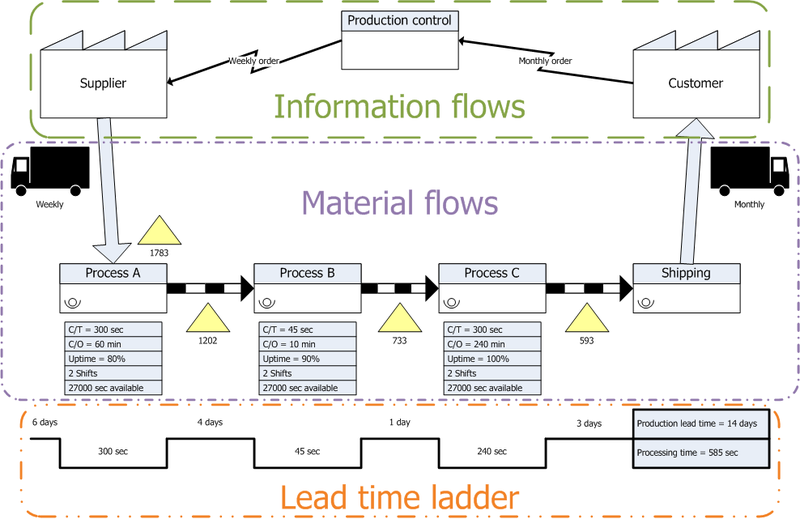
\includegraphics[width=0.7\linewidth]{resources/chapters/OrganizzazioneAziendale/images/vsm.png}
	\centering
	\caption{Esempio di \textit{VSM}}
\end{figure}

\paragraph{Spaghetti Chart}
Il diagramma “a spaghetti” consiste in una rappresentazione grafica degli spostamenti e percorsi compiuti da un prodotto lungo il flusso produttivo. Lo strumento mostra visivamente la linearità o la dispersione dei flussi. Può essere applicato anche per visualizzare gli spostamenti delle persone sul posto di lavoro

\begin{figure}[h!]
	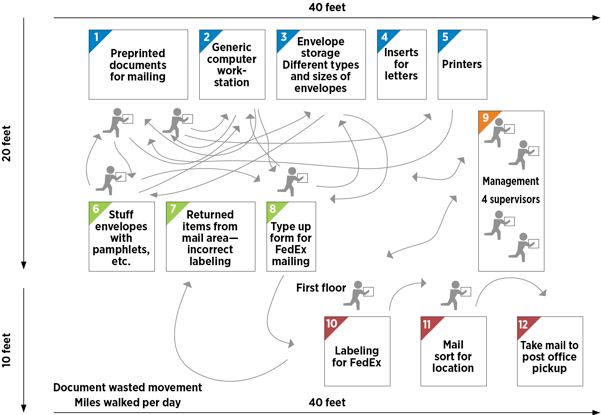
\includegraphics[width=0.8\linewidth]{resources/chapters/OrganizzazioneAziendale/images/spaghetti-chart.png}
	\centering
	\caption{Esempio di \textit{Spaghetti Chart}}
\end{figure}

\paragraph{Kanban}
La parola \textit{kanban} nasce in \textit{Toyota} e vuol dire “cartellino”, in quanto attraverso una gestione a vista di cartellini si evidenziava il consumo e quindi il fabbisogno di rifornimento di materiali alle fasi successive del processo

\begin{figure}[h!]
	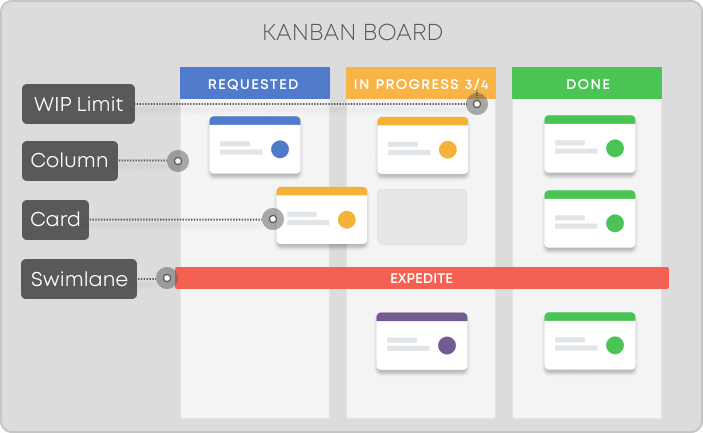
\includegraphics[width=0.8\linewidth]{resources/chapters/OrganizzazioneAziendale/images/kanban.png}
	\centering
	\caption{Esempio di \textit{Kanban}}
\end{figure}

\paragraph{Buffer FIFO}
I \textit{buffer FIFO} sono polmoni a capacità finita nei quali i prodotti avanzano in “fila indiana” garantendo che il primo prodotto che entra sia il primo ad uscire

\begin{figure}[h!]
	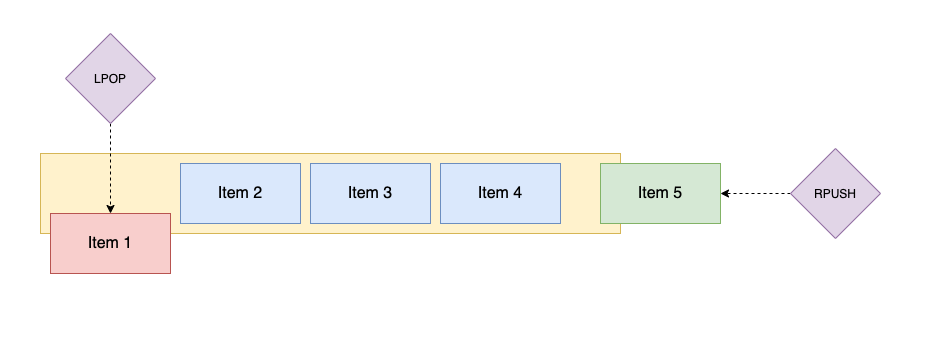
\includegraphics[width=0.8\linewidth]{resources/chapters/OrganizzazioneAziendale/images/fifo.png}
	\centering
	\caption{Esempio di \textit{Buffer Fifo}}
\end{figure}

\paragraph{Total Productive Management}
L’obiettivo del \textit{TPM} (\textit{Total Productive Management}) è quello di ridurre i guasti e le relative attività di manutenzione in emergenza, a favore di manutenzione preventiva (ciclica o su condizione). Il \textit{TPM} richiede inoltre una importante collaborazione del personale di produzione nelle attività di manutenzione autonoma (pulizia, ispezione, ecc...)

\paragraph{Le 5 "S"}
La tecnica \textit{“Five S”} è stata sviluppata in \textit{Toyota} al fine di fornire una guida operativa per l’organizzazione del posto di lavoro, la gestione a vista ed il mantenimento sul posto di lavoro degli standard di ordine e pulizia. Il motto per le \textit{5S} è un posto per ogni cosa ed ogni cosa al suo posto.

L’approccio 5S comporta la realizzazione dei seguenti 5 passi:
\begin{enumerate}
	\item \textbf{Seiri (separare):} separare le cose utili dalle inutili
	\item \textbf{Seiton (sistemare):} identificare e definire l’allocazione delle cose necessarie sul posto di lavoro (materiali, attrezzature, documenti)
	\item \textbf{Seiri (spolverare/pulire):} effettuare una pulizia intelligente del posto di lavoro
	\item \textbf{Seiketsu (standardizzare):} definire gli standard operativi per mantenere ordine e pulizia sul posto di lavoro
	\item \textbf{Shitsuke (seguire le regole):} diffondere gli standard operativi di ordine e pulizia e verificarne il rispetto da parte del personale
\end{enumerate}

\paragraph{Visula Management Systems}
Insieme di tecniche e strumenti per migliorare la gestione a vista sul posto di lavoro (cartellonistica, bacheche, righe a terra, sistemi di controllo stati macchina, sistemi di identificazione materiali/attrezzature, ecc...)


\paragraph{Poka Yoke}
Con il termine \textit{poka yoke} in \textit{Toyota} si identificavano sistemi o procedure che impediscono l’avanzamento nel processo di prodotti difettosi, intercettando gli errori (soprattutto umani) che stanno alla base dei difetti stessi.

Tali sistemi si chiamano anche \textit{“mistake proof”} (a prova d’errore) o \textit{“fool proof”} (a prova di scemo)


